%*********************************************************************
% gdutthesis: 广东工业大学论文模板
% 2022/02/28 v0.1d
%
% 重要提示:
%   1. 请确保使用 UTF-8 编码保存
%   2. 请使用 XeLaTeX 或 LuaLaTeX 编译
%   3. 请仔细阅读用户文档和 Wiki
%   4. 修改、使用、发布本文档请务必遵循 LaTeX Project Public License
%   5. 不需要的注释可以尽情删除
%*********************************************************************
\documentclass[
  % type=doctor
  type=master
  % type=promaster
]{gdutthesis}

% 宏包在这里加载
\usepackage{siunitx}[=v2]
\usepackage{zhlipsum,lipsum}

\gdutsetup{
  style = {
    % cover           = {true},
    cover           = {false},
    open            = {true},
    % open            = {false},
    % font            = {garamond},
    % font            = {libertinus},
    % font            = {lm},
    % font            = {palatino},
    font            = {times},
    % font            = {times*},
    % math-font       = {garamond},
    % math-font       = {libertinus},
    % math-font       = {lm},
    % math-font       = {palatino},
    math-font       = {times},
    % math-font       = {times*},
    cjk-font        = {fandol},
    % cjk-font        = {founder},
    % cjk-font        = {mac},
    % cjk-font        = {sourcehan},
    % cjk-font        = {noto},
    % cjk-font        = {windows},
    % cjk-font        = {none},
    bib-backend     = {bibtex},
    % bib-backend     = {biblatex},
    bib-resource    = {gdutthesis-template.bib},
    bib-style       = {numerical},
    % bib-style       = {author-year},
    % fullwidth-stop  = {mapping},
    % fullwidth-stop  = {catcode},
    fullwidth-stop  = {false},
    hyperlink       = {color},
    % hyperlink       = {border},
    % hyperlink       = {none},
    hyperlink-color = {default},
    % hyperlink-color = {autumn},
    % hyperlink-color = {business},
    % hyperlink-color = {classic},
    % hyperlink-color = {elegant},
    % hyperlink-color = {fantasy},
    % hyperlink-color = {material},
    % hyperlink-color = {science},
    % hyperlink-color = {summer},
    % hyperlink-color = {graylevel},
    % hyperlink-color = {prl},
  },
  theorem = {
    header-font = bf,
    % header-font = sf,
    body-font   = rm,
    % body-font   = kai,
    indent      = cn,
    % indent      = en,
    interval    = dash,
    % interval    = dot,
    braces      = paren,
    % braces      = bracket,
    punct       = colon,
    % punct       = quad,
    qed         = \qedsymbol,
    % qed         = \QED,
  },
  info = {
    title             = {标题},
    title*            = {Title},
    date              = {2020/5/25},
    author            = {张三},
    author*           = {ZHANG San},
    supervisor        = {李四, 教授},
    supervisor*       = {LI Si},
    supervisor-two    = {王五, 教授},
    supervisor-two*   = {WANG Wu},
    supervisor-three  = {none},
    supervisor-three* = {none},
    department        = {自动化学院},
    department*       = {Automation},
    major             = {控制科学与工程},
    student-id        = {2112101234},
    chairman          = {赵六\quad 教授},
    degree            = {工学硕士},
    degree*           = {Master of Engineering Science},
    keywords          = {关键词1, 关键词2, 关键词3, 关键词4},
    keywords*         = {keywords 1, keywords 2, keywords 3, keywords 4},
    secret-level      = {none},
  }
}


\begin{document}

\begin{abstract}
  \zhlipsum[1-4]
\end{abstract}

\begin{abstract*}
  \lipsum[1-4]
\end{abstract*}

\begin{notation}
  \toprule
  符号  & 含义 \\
  \midrule
  $E$   & 能量 \\
  $F$   & 推力 \\
  \bottomrule
\end{notation}

\gduttableofcontents

\mainmatter

\chapter{绪论}{Introduction}

\section{本课题研究背景及研究意义}{Background and significance of research}

\zhlipsum[1]

\section{国内外相关研究现状}{Analysis of the research status at home and abroad}

\subsection{测试}{test}

测试\gdutcite{chendengyuan2000guoshi},测试\gdutcite*{woerdelun2012jingji}。

测试如\autoref{fig:example} 所示,具体参考\autoref{sub-fig-1} 和\autoref{sub-fig-2}。

测试参考\autoref{eq:example}。

测试参考\autoref{tab:example}。

\subsubsection{测试}
测试 test。
\paragraph{测试 test。}
测试 test。
\subparagraph{测试 test。}
测试 test。

\begin{equation}\label{eq:example}
  E = mc^2
\end{equation}

\begin{align}
  E &= mc^2 \\
  mc^2 &= E
\end{align}

\begin{gather}
  E = mc^2 \\
  mc^2 = E
\end{gather}

\begin{figure}
  \subfloat[贴有模板的金属喷嘴示意图]{\label{sub-fig-1}
    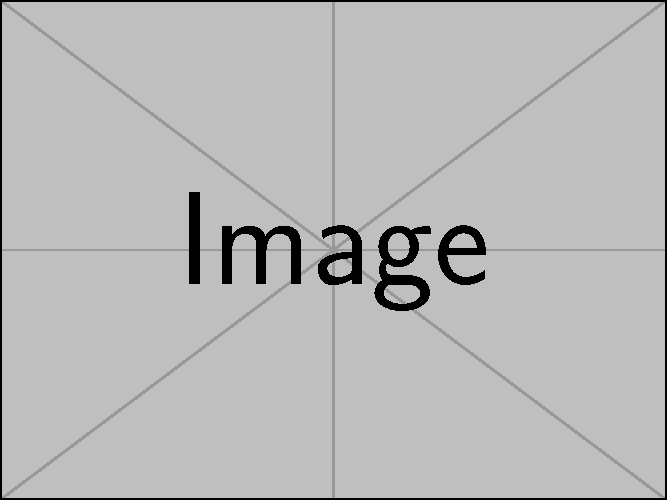
\includegraphics[width=0.4\textwidth]{example-image.pdf}
  }
  \qquad
  \subfloat[由点到线扫描加工原理图]{\label{sub-fig-2}
    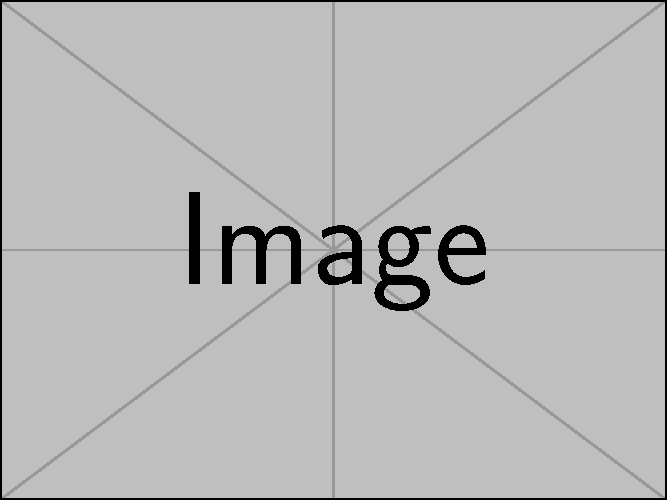
\includegraphics[width=0.4\textwidth]{example-image.pdf}
  }
  \bicaption{模板射流电解加工微沟槽原理图}{Principle of masked jet electrochemical machining of micro grooves}
  \label{fig:example}
\end{figure}

\begin{table}
  \bicaption{DMC5400A 运动控制卡主要技术指标}{DMC5400A main specifications}
  \label{tab:example}
  \begin{tabular}{cc}
    \toprule
    控制卡技术指标              & 具体参数                      \\
    \midrule
    控制电机的脉冲信号频率范围  & $\SI{1}{Hz}\sim\SI{2}{MHz}$   \\
    控制电机的脉冲信号频率精度  & \SI{0.0625}{Hz}               \\
    脉冲信号输出最大电流        & \SI{20}{mA}                   \\
    脉冲信号长度                & 28 位有符号                   \\
    直线插补精度                & $\pm \SI{0.8}{pulse}$         \\
    圆弧插补精度                & $\pm \SI{1.5}{pulse}$         \\
    支持的插补坐标系个数        & 2                             \\
    \bottomrule
  \end{tabular}
\end{table}

\gdutbackmatter
\chapter{结论与展望}{Conclusion and prospect}
\gdutbacksection{研究结论}
\zhlipsum[1]

\gdutbacksection{未来研究展望}
\zhlipsum[1]

\nocite{*}% 列出全部参考文献
\printbibliography

\chapter{攻读学位期间取得与学位论文相关的成果}{Publication and patents during study}

\gdutbacksection{发表和投稿与学位论文相关学术论文}

\begin{results}
  \item \textbf{张三}, 李四, 王五, 等. Jet electrochemical machining of micro dimples with conductive mask.
  Journal of Materials Processing Technology. 2018, 257:101-111. (SCI Impact Factor 3.647,
  WOS:000431161400010)
  \item 李四, \textbf{张三}, 王五, 等. Electrochemical direct-writing machining of micro- channel array.
  Journal of Materials Processing Technology. 2019, 265:138-149. (SCI Impact Factor 3.647,
  WOS:000451935100014)
\end{results}

\gdutbacksection{申请发明专利}

\begin{results}
  \item 李四, \textbf{张三}, 王五. 一种微流道电解加工装置. 发明专利申请号: 201810467763.5.
\end{results}

\gdutstatement

\chapter{致谢}{Acknowlegements}
\zhlipsum[1]

\gdutappendix

\chapter{附录标题}{The appendix title}
对需要收录于学位论文中且又不适合书写于正文中的附加数据、资料、详细
公式推导、计算机程序等有特色的内容,可做为附录排写。
\end{document}